
\chapter{Zahlenr"aume}

\begin{framed}
\subsection*{Worum geht es?}
Bisher haben wir wie selbstverständlich mit Zahlen gerechnet. Dabei haben wir uns keine Gedanken gemacht, welche Gestalt diese Zahlen haben. \\In diesem Abschnitt wollen wir nun mal genauer ansehen, in welche Kategorien man die Zahlen einteilt.
Wie lassen sich verschiedene Zahlen beschreiben/darstellen, gibt es ganz besondere Zahlen? 
\vspace{1cm}
\end{framed}

\section{Die natürlichen Zahlen: $\N$}
Mit den natürlichen Zahlen bist du bereits vertraut. 
Es sind dies die Zahlen:
\begin{center}
$1,2,3,4,...$
\end{center}
\begin{aufgabe}
Es gibt keine grösste natürliche Zahl. Überlege dir wieso dies so ist? Kannst du es sogar schon beweisen?
\end{aufgabe}


\begin{definition}[$\mathbbm{N}$]
Die Menge der \emph{natürlichen Zahlen} ist die unendliche Zahlenmenge \begin{center}$\mathbbm{N}=\{1,2,3,4,...\}$\end{center}
\end{definition}

\subsection{Teilbarkeit}
Eine Zahl ist durch eine andere teilbar, wenn bei der Division kein Rest übrig bleibt, also ein ganzzahliges Resultat auftritt.
\begin{ex} 24 ist durch 8 teilbar, da $\tfrac{24}{8}=3$.\\ Aber 24 ist nicht durch 7 teilbar, denn $\tfrac{24}{7}=3 \text{ Rest 3}$ ($=3 \tfrac{3}{7}$).
\end{ex}
Die Zahl durch welche geteilt werden kann, heisst \emph{Teiler}. Somit ist also 8 ein Teiler von 24, 7 ist jedoch kein Teiler von 24. \\Alle Teiler ausser 1 und der Zahl selber heissen \emph{echte Teiler}.
\begin{aufgabe}[Teilbarkeit]
\begin{center}
\begin{enumerate}[label=\alph*)]
\item Finde alle Teiler von 18, 48, 81?
\item Welche Teiler aus a) sind \emph{echte Teiler}?
\item 32 hat als Teiler unter anderem die 8, die 8 selber hat als ein Teiler die 4.\\
\begin{itemize} \item Kannst du so direkt eine Aussage über die Teilbarkeit von 32 durch 4 angeben? \item Gibt es einen allgemeine Regel?
\end{itemize}
\end{enumerate}
\end{center}
\end{aufgabe}
Betrachten wir den grössten gemeinesamen Teiler und das kleinste gemeinsame Vielfache von natürlichen Zahlen:
\begin{aufgabe}[ggT und kgV bei Zahlen]
\begin{itemize}
\item Wie bestimmt man den ggT und den kgV zweier natürlicher Zahlen? 
\item Welche Verfahren kennst du, wie gehst du genau vor?
\item Finde ggT und kgV von 180 und 210.
\end{itemize}
\end{aufgabe}

\subsection{Primzahlen}
Die \textbf{Primzahlen} sind eine \textit{Untermenge} der natürlichen Zahlen, d.h. sie gehören alle zu den natürlichen Zahlen.
Primzahlen sind bekanntlich alle natürlichen Zahlen, welche \textbf{nur zwei natürliche Zahlen als Teiler} haben. Sie sind also jeweils nur durch \textit{sich selbst }und \textit{1} teilbar. Die kleinsten Primzahlen sind $2, 3, 5, 7, 11, 13, 17, 19...$. 
 Bereits der Grieche \emph{Euklid (ca. 300 v. Chr.)} konnte beweisen, dass es \emph{unendlich} viele Primzahlen gibt.
\begin{aufgabe}[Primzahltest]
\begin{center}
\begin{enumerate}[label=\alph*)]
\item Wie könnte man testen, ob eine gegebene Zahl (z.B. 381) eine Primzahl ist?
\item Kannst du auch eine Idee angeben, wie man alle Primzahlen von 1 bis 1000 findet?
\end{enumerate}
\end{center}
\end{aufgabe}
\subsection{Primfaktorzerlegung}
Eine Zahl kann als Produkt von Teilern geschrieben werden. 
So ist zum Beispiel 30 durch 2, 3, 5, 6, 10 und 15 teilbar (und auch durch sich selbst und 1). Das ergibt folgende Möglichkeiten der Schreibweise von 30 als Produkt von Teilern:
\begin{align*}
(30&=1\cdot 30)\\
30&=2\cdot 15\\
30&=3\cdot 10\\
30&=5\cdot 6
\end{align*}
Wobei das erste Produkt ($1\cdot 30$) nicht sehr interessant ist. Wir wollen uns daher in eine Aufteilung in Teiler ungleich der Zahl selber beschränken.\\
Dieses Aufteilen in zwei Faktoren ist also für jede Zahl möglich, welche \emph{echte Teiler} hat.
Was geschieht, wenn wir die Teiler selber auch noch als Faktoren ausdrücken wollen?
Wenn wir also z.B. bei $30=2\cdot 15$ die 15 auch noch weiter in Teiler aufteilen wollen. 15 hat als \emph{echte Teiler} 3 und 5, lässt sich also schreiben als $15=3\cdot 5$.\\
Somit erhalten wir $30=2\cdot 3\cdot 5$.\\
Dieses Zerlegen in Faktoren kann man soweit ausführen, bis jeder einzelne Faktor eine Primzahl ist, welche sich nicht weiter zerlegen lässt. Der folgende Satz sagt aus, dass es egal ist in welcher Reihenfolge wir zerlegen.

\begin{satz}[Primfaktorzerlegung]
Eine natürliche Zahl hat eine \textbf{eindeutige Zerlegung} in Primfaktoren, d.h. in Faktoren, welche alle Primzahlen sind.
\end{satz}

Die Primfaktorzerlegung lässt sich am einfachsten bestimmen, indem man nacheinander durch die Primzahlen, beginnend mit $2$, teilt und Teiler als Faktoren hinschreibt.
\begin{ex}
Wir wollen die Primfaktorzerlegung von $378$ bestimmen. Also teilen wir zuerst durch $2$, es bleibt $189$ übrig. Dann versuchen wir mit $189$ nochmals durch $2$, was aber nicht ohne Rest geht. Deshalb versuchen wir durch die $3$ und sehen, dass dies geht, wir erhalten 63. Wir versuchen nochmals durch $3$ und sehen, dass dies nochmals geht, mit Quotient $21$. Wir versuchen nochmals die 3, was nochmals geht mit Quotient $7$. Schliesslich wissen wir, dass 7 selber eine Primzahl ist und schreiben sie direkt als letzten Faktor auf. Formal aufgeschrieben, sieht der Ablauf für das Beispiel $378$ so aus:
\begin{align*}
378&=2\cdot 189\\
&=2\cdot 3\cdot 63\\
&=2\cdot 3 \cdot 3\cdot 21\\
&=2\cdot 3 \cdot 3 \cdot 3 \cdot 7
\end{align*}

\end{ex}
\begin{aufgabe}[Primfaktorzerlegung]
Zerlege in die Primfaktoren und schreibe den Ablauf wie in obigem Beispiel auf:
\begin{center}
\begin{enumerate}[label=\alph*)]
\item 616
\item 2310
\item 182
\end{enumerate}
\end{center}
\end{aufgabe}

Im Fach Mathematik wollen wir möglichst exakt sein. Das Verfahren zum Berechnen einer Primfaktorzerlegung wollen wir also in Form eines \textbf{Algorithmus} (d.h. einer \textit{eindeutigen Handlungsvorschrift zur Lösung eines Problems}) darstellen.\\
Einen Algorithmus kann man einem Computer beibringen (d.h. \textit{programmieren}), der uns dann für jede Eingabe sehr schnell die Primfaktorzerlegung berechnet.
\begin{howto}
\begin{center}
	\begin{minipage}[t]{11cm}
		\begin{algorithm*}[H]

%			\SetKwInParam{Func}{(}{)}
			\SetKwInOut{Input}{Eine Zahl}
			\SetKwData{Left}{Primfaktorzerlegung der Zahl}
			\Ein{Eine Zahl} \Aus{Primfaktorzerlegung der Zahl}
			Rest=Zahl\;
			Primzahl=2\;
			Primfaktoren=$\emptyset$\;
			\While{Rest keine Primzahl}{
			\If{Rest teilbar durch Primzahl}
			{Primfaktoren=Primfaktoren $\cup$ Primzahl\;
			Rest$\leftarrow$ Rest/Primzahl\;}
			\Else{Primzahl = naechste Primzahl\;}
			}
			\Return{Primfaktoren $\cup$ Rest\;}
			\caption{Primfaktorzerlegung}
		\end{algorithm*}
	\end{minipage}
\end{center}
\end{howto}\newpage
\section{Die ganzen Zahlen: $\mathbbm{Z}$}

\begin{definition}[$\mathbbm{Z}$]
Die Menge der \emph{ganzen Zahlen} ist die unendliche Zahlenmenge \begin{center}$\mathbbm{Z}=\{...,-4,-3,-2,-1,0,1,2,3,4,...\}$\end{center}
\end{definition}


$\mathbbm{N}$ ist also eine echte Teilmenge der ganzen Zahlen $\mathbbm{Z}$.
\begin{align*}
\mathbbm{N} \subset \mathbbm{Z}
\end{align*}

\begin{figure}[H] 
\center{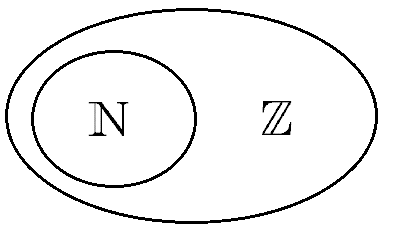
\includegraphics[scale=0.35]{1_Zahlenraeume/ninz.png}}
\end{figure}
\section{Die rationalen Zahlen: $\mathbbm{Q}$}

Mit den natürlichen und ganzen Zahlen lassen sich Brüche schreiben. Diese Brüche sind eine eigene Klasse von Zahlen:

\begin{definition}[$\mathbbm{Q}$]
Die Menge der \emph{rationalen Zahlen} ist die unendliche Zahlenmenge aller gewöhnlichen Brüche. D.h. aller Zahlen, welche als Brüche geschrieben werden können mit Zähler aus $\mathbbm{Z}$ und Nenner aus $\mathbbm{N}$.
\end{definition}
\begin{ex}
Jede ganze Zahl ist sicherlich in $\mathbbm{Q}$, wir können ja beispielsweise 3 mit $\tfrac{3}{1}$ auch als Bruch darstellen.
Es gilt also sicherlich:

\begin{figure}[H] 
\center{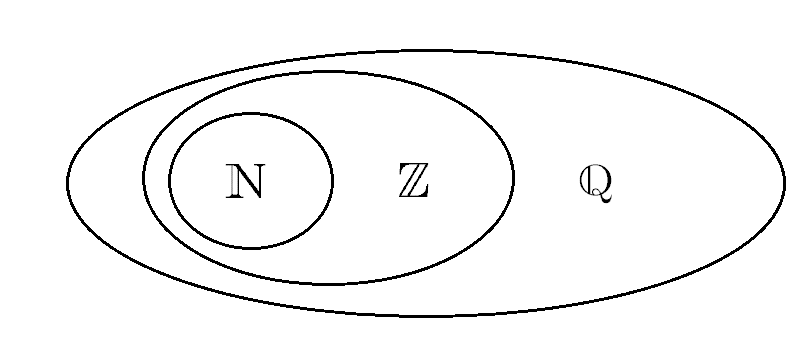
\includegraphics[scale=0.35]{1_Zahlenraeume/ninzinq.png}}
\end{figure}

\end{ex}
\begin{ex}
Weitere Beispiele für Zahlen aus $\mathbbm{Q}$ sind $\tfrac{1}{3}$, $\tfrac{27}{2}$, $-\tfrac{157}{3921}$.
\end{ex}
Statt dem (gekürzten) Bruch, können wir Zahlen aus $\mathbbm{Q}$ in \textit{Dezimalschreibweise} angeben. Die Schreibweise mit einem Strich über einer (oder mehreren) Zahl(en) bedeutet, dass die Dezimaldarstellung endlos lange mit dieser Zahl (bzw. Zahlen) wiederholt fortgesetzt wird (werden). Zahlen, welche eine solche endlos wiederholte Ziffernfolge haben, nennt man \emph{periodisch}.
\begin{ex}
$\tfrac{1}{3}=0.\overline{3}=0.33333...$, $\tfrac{3}{7}=0.\overline{428571}=0.428571428571428571...$
\end{ex}
\begin{aufgabe}
Welche der folgenden Zahlen besitzen eine \textit{endliche}, welche eine \textit{periodische} Dezimaldarstellung?
\begin{enumerate}[label=\alph*)]
\begin{multicols}{2}
\item $\tfrac{1}{4}$
\item $\tfrac{1}{13}$
\item  $\tfrac{1}{20}$
\item  $\tfrac{19}{24}$
\end{multicols}
\end{enumerate}
\end{aufgabe}

\begin{satz}[Dezimaldarstellung von Zahlen aus $\mathbbm{Q}$] Jede rationale Zahl besitzt eine \textbf{endliche oder periodische Dezimaldarstellung}. Umgekehrt kann jede Zahl mit einer  \textbf{endlichen oder periodischen Dezimaldarstellung} auch als Bruch geschreiben werden. (ohne Beweis)
\end{satz}

Der Satz besagt also, dass jeder Bruch entweder eine endliche (z.B. $\tfrac{1}{2}=0.5$) oder eine periodische Dezimaldarstellung hat (z.B. $\tfrac{1}{3}=0.\overline{3}$) und dass genau diese Zahlen mit einer solchen Darstellung auch gleich alle Bruchzahlen sind. In manchen Lehrbücher, auch in Algebra 1 von Deller/Gebauer/Zinn, wird diese Eigenschaft als definierende Charakteristik der rationalen Zahlen verwendet.\\
Gibt es auch Zahlen, welche keine endliche oder periodische Dezimaldarstellung besitzen? Also Zahlen mit scheinbar zufälliger, nie endender Zahlenfolge in der Dezimaldarstellung.
Die Antwort lautet "`Ja"' und führt uns auf die letzte Klasse von Zahlen, wodurch der Zahlenstrahl kompletiert wird.
\section{Die reellen Zahlen: $\mathbbm{R}$}
\subsection{Definition und Übersicht} 
Neben den Zahlen, welche als Bruch dargestellt werden können, gibt es spezielle Zahlen, welche \textbf{nicht als Bruch} geschrieben werden können.
Diese Klasse nennt man \textit{irrationale Zahlen}:

\begin{definition}[$\mathbbm{I}$]
Die Menge der \emph{irrationalen Zahlen} $\mathbbm{I}$ ist die unendliche Zahlenmenge aller \textbf{nicht als Brüche darstellbarer Zahlen}.
\end{definition}

\begin{ex}
Die Zahl $\pi=3.141592...$ besitzt keine endliche oder periodische Dezimaldarstellung, ist also gemäss obigem Satz nicht als Bruch darstellbar. Somit gehört $\pi$ zu den irrationalen Zahlen. Nach heutigem Wissensstand kommt jede beliebige Zahlenfolge unendlich oft in den Nachkommastellen von $\pi$ vor. So finden sich viele Geburstage als Zahlenfolge bereits in den ersten 200 Mio. Stellen nach dem Komma. Die Zahlenfolge \texttt{24121998} (für den Geburtstag 24.12.1998) kommt beispielsweise an der 109477334. Position nach dem Komma vor. Und ist umrandet von \texttt{1569235231} 24121998 \texttt{5876694267}. (Quelle: \url{http://www.angio.net/pi/}).
\end{ex}
\begin{ex}
Viele Wurzeln sind nicht als Brüche darstellbar. So beispielsweise $\sqrt{2}$ und $\sqrt{5}$. 
Legenden besagen, dass die Entdeckung der Irrationalität von $\sqrt{5}$ bei den Anhängern Pythagoras zu einer tiefen Sinnkrise geführt hat.
Wir werden im folgenden Abschnitt die Irrationalität von $\sqrt{2}$ beweisen.
\end{ex}

Nun haben wir also Zahlen gesehen, welche als Brüche darstellbar sind (die rationalen Zahlen $\mathbbm{Q}$) und solche, welche man nicht als Brüche schreiben kann (die irrationalen Zahlen $\mathbbm{I}$). Zusammen haben wir so alle Zahlen auf dem Zahlenstrahl kennengelernt:

\begin{definition}[$\mathbbm{R}$]
Die Menge der \emph{reellen Zahlen} $\mathbbm{R}$ ist die unendliche Zahlenmenge aller Zahlen auf dem Zahlenstrahl. Sie bildet also die Vereinigung von rationalen Zahlen und irrationalen Zahlen.
\end{definition}
Jeder Punkt auf dem Zahlenstrahl entspricht einer reellen Zahl und umgekehrt.
Skizze mit einigen Beispielzahlen:
\begin{framed}
\vspace*{2cm}
\end{framed}

In Mengenschreibweise ergibt sich folgendes Bild:
\begin{figure}[H] 
\center{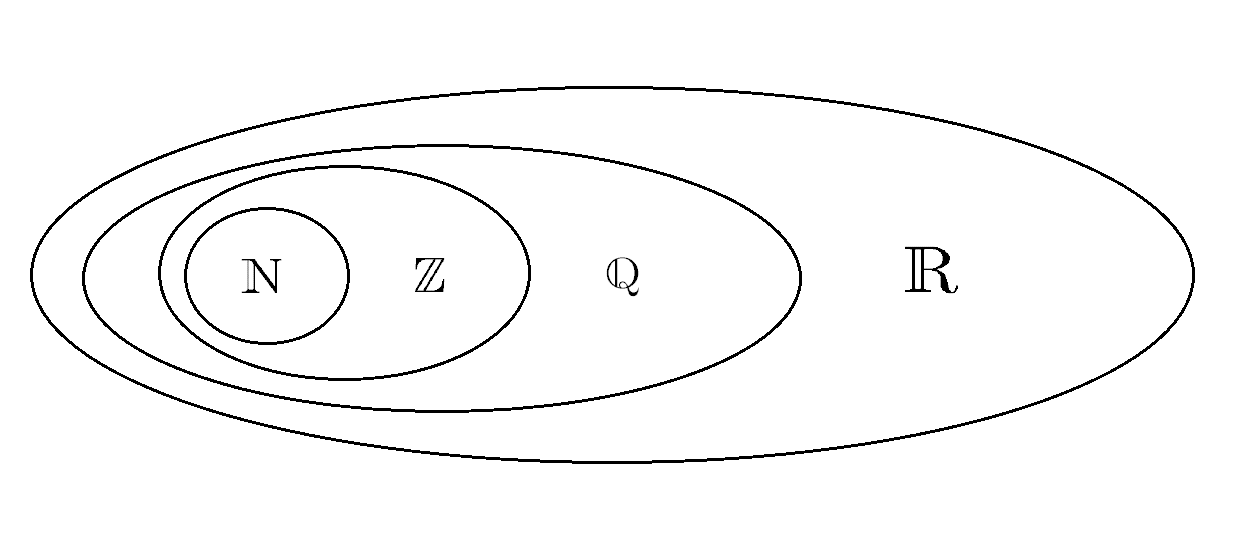
\includegraphics[scale=0.35]{1_Zahlenraeume/nzqir.png}}
\end{figure}

%\begin{aufgabe} [Üben!]
%Beschreibe die folgenden Zahlenmengen und gebe, wo möglich, jeweils zwei Beispiele an.
%\begin{enumerate}[label=\alph*)]
%\begin{multicols}{3}
%\item $\mathbbm{R}\setminus\mathbbm{Q}$
%\item $\mathbbm{Q}\setminus\mathbbm{R}$
%\item $\mathbbm{Z}\setminus\mathbbm{N}$
%\item  $\mathbbm{R}\setminus\mathbbm{Z}$
%\item  $\mathbbm{R}\setminus\mathbbm{I}$
%\item $\mathbbm{I}\setminus\mathbbm{Q}$
%\end{multicols}
%\end{enumerate}
%\end{aufgabe}

\subsection{Irrationalität von Wurzel 2}
Wir wollen in diesem Abschnitt zeigen, dass die Wurzel aus 2 irrational ist.
Wieso betrachten wir diesen Beweis, dazu gibt es mehrere Gründe:
\begin{itemize}
\item Um zu zeigen, dass $\sqrt{2}$ keine rationale Zahl ist.
\item Um einzusehen, dass das System der rationalen Zahlen $\mathbbm{Q}$ nicht perfekt ist.
\item Um ein Beispiel eines \textit{indirekten Beweises} zu sehen.
\end{itemize}
Bei einem \textit{indirekten Beweises} macht man zuerst eine Annahme. Dann zeigt man, dass diese Annahme einen Widerspruch ergibt. Dadurch weiss man, dass die Annahme falsch gewesen sein muss. .\\

Beginnen wir jedoch zuerst mit einer geometrischen Bestimmung von $\sqrt{2}$

Die Fläche eines Quadrats ist die Seitenlänge im Quadrat. Also hat zum Beispiel ein Quadrat mit Seitenlänge 1 die Fläche 1.
Will man ein Quadrat mit Fläche 2, so kann man dies folgendermassen aus einem Quadrat mit Fläche 1 konstruieren.\\
Skizze: (Wobei 1 $\approx$ 2 Häuschen $\approx$ ... cm)
\begin{framed}
\begin{figure}[H] 
\center{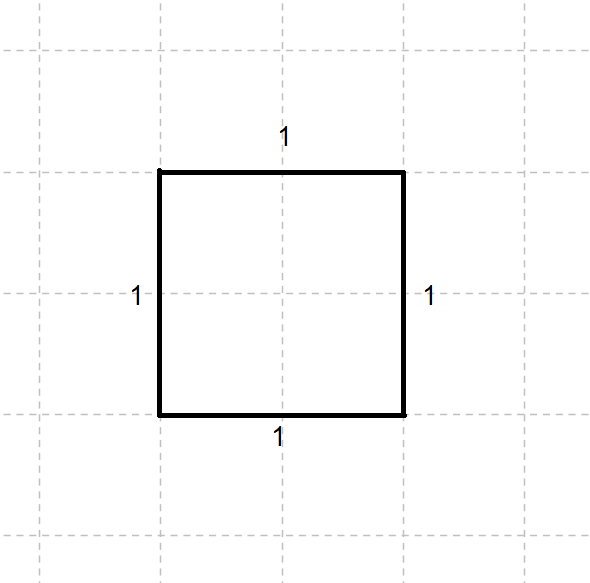
\includegraphics[scale=0.5]{1_Zahlenraeume/wurzel2fs.png}}
\end{figure}
\end{framed}
Die Seitenlänge dieses Quadrats ist nun also $\sqrt{2}$. \\
Rechnerisch können wir $\sqrt{2}$ ebenso bestimmen.
Dazu benutzen wir das Heron Verfahren. Betrachten wir zur Herleitung der Idee zunächst dessen geometrische Veranschaulichung.
\newpage\noindent
\textbf{Heron Verfahren zur nummerischen Bestimmung von Quadratwurzeln (geometrisch)}:
\begin{figure}[H] 
\center{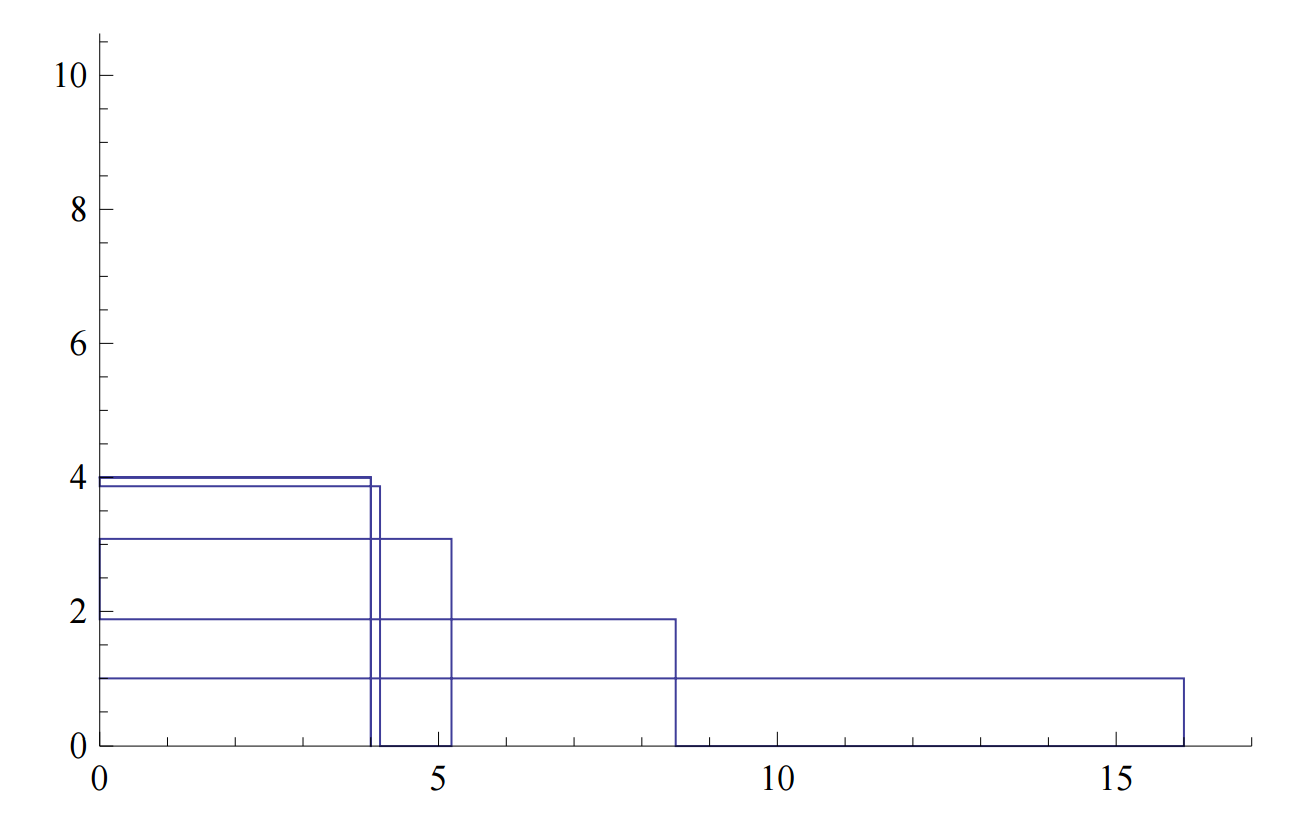
\includegraphics[scale=0.5]{1_Zahlenraeume/heron16.png}}
\caption{Illustration: Heron Verfahren für Wurzel 16}
\end{figure}
%https://www.mathi.uni-heidelberg.de/~thaeter/anasem08/Heron
\newpage\noindent
\textbf{Heron Verfahren zur nummerischen Bestimmung von Wurzel 2 (rein rechnerisch)}:
\begin{framed}
%http://www.arndt-bruenner.de/mathe/scripts/heronframe.htm
\vspace{9cm}
\end{framed}
\noindent

\begin{aufgabe}[Heron-Verfahren]
Beschreibe das obige Heron-Verfahren algorithmisch, d.h. in einer Art Kochrezept und fülle dieses in untenstehendes Feld ein. 
\end{aufgabe}
\begin{howto}[Heron-Verfahren zur Berechnung von $\sqrt{2}$]
\begin{center}
	\vspace{6cm}
\end{center}
\end{howto}
Nun wollen wir noch beweisen, dass Wurzel 2 tatsächlich irrational ist.\newpage\noindent
\textbf{Beweis, dass $\sqrt{2}$ irrational (nach Euklid):}\\
Wir machen die:
\textbf{Annahme:} $\sqrt{2}$ ist rational, lässt sich also als gekürzter Bruch $\sqrt{2}=\tfrac{p}{q}$ mit $p$ und $q$ aus $\mathbbm{N}$ schreiben.\\
Dann gilt:
\begin{align*} 2&=(\sqrt{2})^2=(\tfrac{p}{q})^2
\end{align*}
Also ist $p^2=2\cdot q^2$ und somit $p^2$ eine gerade Zahl, und daher ist $p$ selber auch \textbf{gerade}. Wir können also $p$ schreiben als $p=2\cdot a$
Da nun aber auch:
\begin{align*} q^2&=\tfrac{p^2}{2}\\
&=\tfrac{(2\cdot a)^2}{2}\\
&=\tfrac{4\cdot a^2}{2}\\
&=2\cdot a^2
\end{align*}
Somit ist auch (mit gleicher Begründung wie für $p$) $q$ gerade.
Also kann $\tfrac{p}{q}$ kein ungekürzter Bruch sein und die \textbf{Annahme} dass $\sqrt{2}$ rational ist, ist somit \textbf{falsch}.
Also ist $\sqrt{2}$ irrational.
\subsection*{Wie sieht es mit andern Wurzelzahlen aus?}
Um andere Wurzelzahlen zu betrachten, wollen wir zuerst noch die Primfaktorzerlegung der natürlichen Zahlen auf die rationalen Zahlen ausweiten. Wir können uns die rationale Zahl schon ganz gekürzt vorstellen, so haben wir als Nenner eine natürliche Zahl $q$, für welche wir bereits die Primfaktorzerlegung kennen, und über dem Strich ebenso eine ganze Zahl $p$, welche wir in Primfaktoren zerlegen können.\\
Kann ein Faktor sowohl im Nenner, als auch im Zähler vorkommen?\\
Nein, denn sonst könnte man die beiden ja wegkürzen.\\
Also haben wir folgende Form der Primfaktorzerlegung.

\begin{definition}[Primfaktor"-zerlegung einer rationalen Zahl ]
\begin{align*}
z=\pm 2^{k_2} \cdot 3^{k_3} \cdot 5^{k_5} \cdot 7^{k_7} \cdot {11}^{k_{11}}\cdots
\end{align*}
mit
\begin{itemize}
\item Vorzeichen + oder -.
\item ganzzahligen Exponenten, also $k_2, k_3, k_5, k_7, k_{11}... \in \mathbbm{Z}$
\item Produkt über alle Primzahlen, wobei diejenigen mit Exponenten 0 nicht geschrieben werden müssen.
\end{itemize} 
\end{definition}
Diese Primfaktorzerlegung ist eindeutig, d.h. jeder gekürzte Bruch hat genau eine solche Darstellung.\vspace{-0.5cm}
\begin{ex}
\begin{align*}
-\frac{12}{25}&=-\frac{2^2\cdot 3}{5^2}=-2^2\cdot 3\cdot 5^{-2}\\
\frac{56}{81}&=\frac{2^3\cdot 7}{3^4}=2^3\cdot 3^{-4}\cdot 7
\end{align*}
\end{ex}
\begin{aufgabe}
Berechne die Primfaktorzerlegung von:
\begin{enumerate}[label=\alph*)]
\begin{multicols}{2}
\item $-\tfrac{15}{154}$
\item $\tfrac{385}{512}$
\end{multicols}
\end{enumerate}
\end{aufgabe}
Was geschieht, wenn wir nun eine Zahl $z$ aus $\mathbbm{Q}$ quadrieren?\\
Wir sehen, dass sich die Anzahl eines jeden Faktors verdoppelt. 
\begin {align*}
z^2=2^{2 k_2} \cdot 3^{2 k_3} \cdot 5^{ 2k_5} \cdot 7^{2 k_7} \cdot {11}^{2 k_{11}}\cdots
\end{align*}
\begin{framed}
Daher sind die Quadrate von rationalen Zahlen genau die Zahlen mit:
\begin{itemize}
\item lauter geraden Exponenten in der Primfaktorzerlegung
\item und einem positiven Vorzeichen.
\end{itemize}\end{framed}
Umgekehrt können wir so für die Wurzeln von rationalen Zahlen folgern, dass:
\begin{satz}
Die Wurzel einer rationalen Zahl $q$ ist genau dann \textbf{auch rational}, falls:
\begin{itemize}
\item in der Primfaktorzerlegung  \textbf{lauter gerade Exponenten} vorkommen oder 0
\item und die Zahl $q$ positiv ist.
\end{itemize}
Ist mindestens \textbf{einer der Exponenten ungerade}, dann ist die Wurzel $x =\sqrt{q}$ eine \textbf{irrationale }Zahl.
\end{satz}
\begin{ex}
$2^6\cdot 3^{-8}\cdot 7^2$ ist das Quadrat von $z=2^3\cdot 3^{-4}\cdot 7$, denn $z^2=(2^3\cdot 3^{-4}\cdot 7)\cdot (2^3\cdot 3^{-4}\cdot 7)=2^6\cdot 3^{-8}\cdot 7^2$
\end{ex}
\begin{ex}
Die Zahl 5 hat die Primfaktorzerlegung $5=5^1$. Wegen dem ungeraden Exponenten 1 kann 5 nicht das Quadrat einer rationalen Zahl sein.
\end{ex}

\begin{ex}
$n=16$ hat die Primfaktorzerlegung $n=2^4$, der Exponent 4 ist gerade, somit ist $\sqrt{16}$ eine ganze Zahl. 
\end{ex}\vspace{-0.3cm}
\begin{ex}
$n=1200$ hat die Primfaktorzerlegung $n=2^4\cdot 3 \cdot 5^2$, der Exponent von 3 ist ungerade, somit ist $\sqrt{1200}$ eine irrationale Zahl. 
\end{ex}

Zu Aufgabe 10 und 11 findest du die Bezeichungen auf Seite 2 unten.
\begin{buchaufgabe}
Löse im Buch Algebra 1, die Aufgaben 6, 9, 10, 63.
\end{buchaufgabe}

\begin{aufgabe}
Löse im Buch Algebra 1, die Aufgaben 7, 11.
Sowie Aufgabe 65: Schreibe in a) und b) die Dezimalzahlen als Bruch und betrachte die Primzahlzerlegung von Zähler und Nenner.
\end{aufgabe}
\begin{figure}[H] 
\center{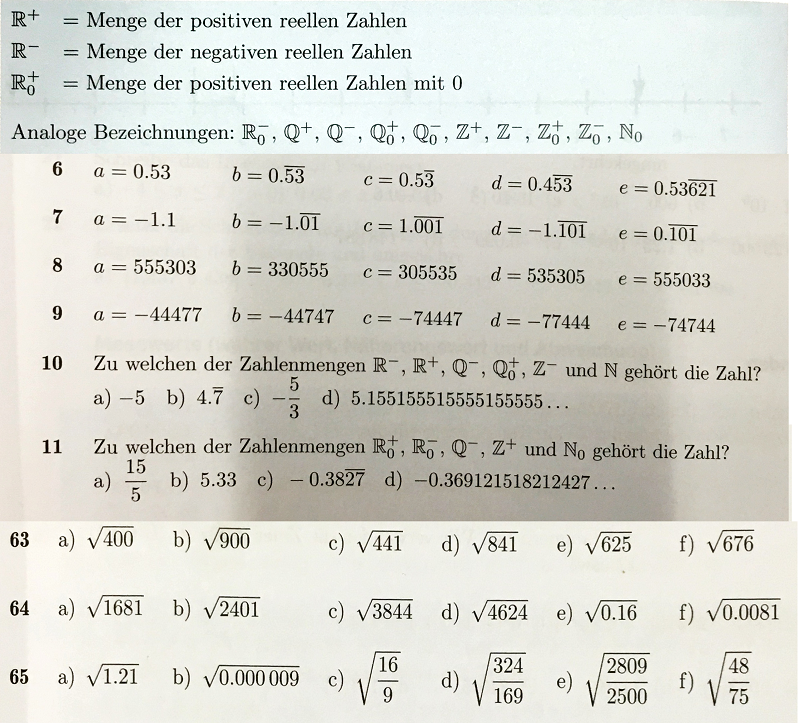
\includegraphics[width=\textwidth]{1_Zahlenraeume/aufgaben.png}}
\end{figure}
\newpage
\section{Intervallschreibweise}

Intervalle sind Mengen von Zahlen, die zwischen zwei Grenzen liegen. Die genaue Bezeichnung hängt davon ab, ob die Grenzen dazugehören oder nicht:\\
\begin{center}
\begin{tabular}{c|c}
Schreibweise & Eigenschaft der Elemente\\\hline
$[3,4]$& $3 \leq x\leq 4$\\\hline
$]3,4[$& $3 < x < 4$\\\hline
$ [7.1,8.2[$& $7.1\leq x < 8.2$\\\hline
$]7.1,8.2]$& $7.1 < x \leq 8.2$
\end{tabular}
\end{center}
\begin{aufgabe}
Löse im Buch Algebra 1, Seite 5 Aufgabe 20 und 21
\end{aufgabe}
\begin{aufgabe}
Löse auf Seite 84 die Aufgabe 73, 76 und 79.
\end{aufgabe}
\section{Betrag einer Zahl}
Zum Ende dieses Kapitel betrachten wir noch eine Funktion auf Zahlen, welche jeweils den Abstand zu 0 auf der Zahlengerade ausgibt:

\begin{definition}[Betrag einer Zahl]
Der \emph{Betrag einer Zahl} ist definiert als:
\begin{align*}
|x|= \begin{cases} 
\phantom{-} x & \text{falls } x \geq 0\\
-x & \text{falls } x<0
\end{cases}
\end{align*}
\end{definition}


\begin{aufgabe}[Betragsfunktion üben]
Löse Aufgabe 60 und 61 aus dem Algebra 1 Buch:



\end{aufgabe}

\subsection*{Rückblick}
In diesem Kapitel hast du die Zahlenräume kennengelernt. Du hast die natürlichen Zahlen $\mathbbm{N}$, ganzen Zahlen $\mathbbm{Z}$, rationalen Zahlen $\mathbbm{Q}$, irrationalen Zahlen $\mathbbm{I}$ und als Gesamtheit die reellen Zahlen $\mathbbm{R}$ kennengelernt. Dabei hast du die Wurzel von 2 als Beispiel einer irrationalen Zahl gesehen und dazu einen Beweis. Mithilfe der Primfaktorzerlegung konnten wir schliesslich eine ganze Klasse von Zahlen angeben, deren Wurzel irrational ist.